\chapter{Appendix}
\section{Signal Processing Basics}
A signal is a function that conveys information about the behavior or attributes of some phenomenon.
In the physical world, any quantity exhibiting variation in time or variation in space (such as an image) is potentially a signal that might provide information on the status of a physical system, or convey a message between observers.

The Fourier Transform is an important image processing tool which is used to decompose an image into its sine and cosine components. The output of the transformation represents the image in the Fourier or frequency domain, while the input image is the spatial domain equivalent. In the Fourier domain image, each point represents a particular frequency contained in the spatial domain image. 

\subsection{Fourier Transformation}
The Fourier-Transform is a mathematical tool which allows to transform a given function or rather a given signal from defined over a time- (or spatial-) domain into its corresponding frequency-domain.
 
Let $f$ an measurable function over $\mathds{R}^n$. Then, the continuous Fourier Transformation(\textbf{FT}), denoted as $\mathcal{F}\{f\}$ of $f$, ignoring all constant factors in the formula, is defined as:
 
\begin{equation}
  \mathcal{F}_{FT}\{f\}(w) = \int_{\mathds{R}^n} f(x)e^{-iwt} dt
  \label{eq:cft}
\end{equation}

whereas its inverse transform is defined like the following which allows us to obtain back the original signal:

\begin{equation}
  \mathcal{F}_{FT}^{-1}\{f\}(w) = \int_{\mathds{R}} \mathcal{F}\{w\}e^{iwt} dt
  \label{eq:icft}
\end{equation}

Usual $w$ is identified by the angular frequency which is  equal $w = \frac{2 \pi}{T} = 2 \pi v_f$. In this connection, $T$ is the period of the resulting spectrum and $v_f$ is its corresponding frequency.

By using Fourier Analysis, which is the approach to approximate any function by sums of simpler trigonometric functions, we gain the so called Discrete Time Fourier Transform (in short \textbf{DTFT}). The DTFT operates on a discrete function. Usually, such an input function is often created by digitally sampling a continuous function. The DTFT itself is operation on a discretized signal on a continuous, periodic frequency domain and looks like the following:

\begin{equation}
  \mathcal{F}_{DTFT}\{f\}(w) = \sum_{-\infty}^{\infty} f(x) e^{-iwk}
  \label{eq:dtft}
\end{equation}

Note that the DTFT is not practically suitable for digital signal processing since there a signal can be measured only in a finite number of points. Thus, we can further discretize the frequency domain and will get then the Discrete Fourier Transformation (in short \textbf{DFT}) of the input signal:

\begin{equation}
  \mathcal{F}_{DFT}\{f\}(w) = \sum_{n=0}^{N-1} f(x) e^{-iw_{n}k}
  \label{eq:dft}
\end{equation}

Where the angular frequency $w_n$ is defined like the following $w_n = \frac{2\pi n}{N}$ and $N$ is the number of samples within an equidistant period sampling.

Any continuous function $f(t)$ can be expressed as a series of sines and cosines. This representation is called the Fourier Series (denoted by $FS$) of $f(t)$.
\begin{equation}
  f(t) = \frac{1}{2}a_0 + \sum_{n=1}^{\infty} a_n cos(nt) + \sum_{n=1}^{\infty} b_n cos(nt)
  \label{eq:dfs}
\end{equation}

where

\begin{align}
    a_0 = \int_{-\pi}^{\pi} f(t) dt \nonumber \\
    a_n = \frac{1}{\pi}\int_{-\pi}^{\pi} f(t) cos(nt) dt \nonumber \\
    b_n = \frac{1}{\pi}\int_{-\pi}^{\pi} f(t) sin(nt) dt
\end{align}

\begin{figure}[H]
  \centering
  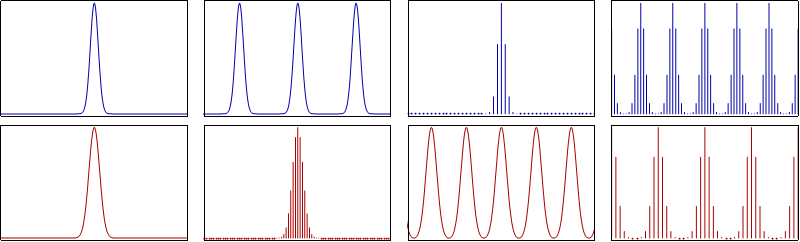
\includegraphics[scale=0.5]{background/dcft.png}
  \caption[]{Relationship$\footnotemark$ between the continuous Fourier transform and the discrete Fourier transform: Left column: A continuous function (top) and its Fourier transform $\ref{eq:cft}$ (bottom). Center-left column: Periodic summation of the original function (top). Fourier transform (bottom) is zero except at discrete points. The inverse transform is a sum of sinusoids called Fourier series $\ref{eq:dfs}$. Center-right column: Original function is discretized (multiplied by a Dirac comb) (top). Its Fourier transform (bottom) is a periodic summation (DTFT) of the original transform. Right column: The DFT $\ref{eq:dft}$ (bottom) computes discrete samples of the continuous DTFT $\ref{eq:dtft}$. The inverse DFT (top) is a periodic summation of the original samples.}
\label{fig:contdiscft}
\end{figure}
\footnotetext{image of illustration has been taken from \href{http://en.wikipedia.org/wiki/Discrete_Fourier_transform}{wikipedia}}

\begin{table}[H]
    \begin{tabular}{l|l|l}
    \hline
    Spetail signal $f(t)$ is & Operator & Transformed frequency signal $\hat{f}(\omega)$ is\\
    \hline
    continuous and periodic in $t$ & FS $\ref{eq:dfs}$ & only discrete in $\omega$ \\
    only continuous in $t$ & FT $\ref{eq:cft}$ & only continuous in $\omega$\\
    only discrete in $t$ & DTFT $\ref{eq:dtft}$ & continuous and periodic in $\omega$\\
    discrete and periodic in $t$ & DFT $\ref{eq:dft}$ & discrete and periodic in $\omega$\\
    \hline
    \end{tabular}
\caption{Fourier operator to apply for a given spatial input signal and the properties of its resulting output signal in frequency space}
\label{tab:ftoperatorsdependencies}
\end{table}

\subsection{Convolution}
The convolution $f*g$ of two functions $f$, $g$$\colon \mathds{R}^n \to \mathds{C} $ is defined as:  
\begin{equation}
  \mathcal (f*g)(t) = \int_{\mathds{R}^n} f(t)g(t-x) dx
  \label{eq:convolution}
\end{equation}

Note that the Fourier transform of the convolution of two functions is the product of their Fourier transforms. This is equivalent to the fact that Convolution in spatial domain is equivalent to multiplication in frequency domain. Therefore, the inverse Fourier transform of the product of two Fourier transforms is the convolution of the two inverse Fourier transforms.
Last an illustration of the relationships between the previous presented Fourier transformations and different given input signals. First an concrete example shown in Figure $\ref{fig:contdiscft}$. Table $\ref{tab:ftoperatorsdependencies}$ tells what Fourier transformation operator has to be applied to which kind of input signal and what properties its resulting Fourier transform will have.

\subsection{Taylor Series}
Taylor series is a representation of a function as an infinite sum of terms that are calculated from the values of the function's derivatives at a single point.

The Taylor series $\mathcal T$ of a real or complex-valued function $f(x)$ that is infinitely differentiable at a real or complex number $a$ is the power series:

\begin{equation}
  \mathcal T(f;a)(x) = \sum_{n=0}^{\infty} \frac{f^{n}(a)}{n!}(x-a)^n
  \label{eq:deftaylor}
\end{equation}